% CounterClockwise-Only Steering Robot -- Detour Steer algorithm
% Typeset in the MDPI journal style (rule / caption / rule / boxed body / rule)
% Build:  pdflatex algorithm.tex

\documentclass[11pt,a4paper]{article}

\usepackage[T1]{fontenc}
\usepackage[top=1.5cm,bottom=1.5cm,left=1.9cm,right=1.9cm]{geometry}
\usepackage{mathpazo}                       % Palatino, as used by MDPI
\usepackage{amsmath}
\usepackage{amssymb}
\usepackage{needspace}
\usepackage{booktabs}
\usepackage[linesnumbered,lined]{algorithm2e}
\usepackage{graphicx}

% ---------------------------------------------------------------- styling ---
\RestyleAlgo{boxed}                         % frame around the body only
\SetAlgoNlRelativeSize{-1}                  % slightly smaller line numbers

\newcommand{\algcommentfont}[1]{\footnotesize\textnormal{#1}}
\SetCommentSty{algcommentfont}
\SetKwComment{tcp}{/\kern-0.12em/\ }{}      % "//" without the Palatino gap
\SetFuncSty{textit}
\SetArgSty{textnormal}                      % constants and strings stay upright

% caption block: thick rule / title / thin rule  ... body ...  thick rule
\newcommand{\algohead}[3][62mm]{%
  \Needspace*{#1}%
  \par\addvspace{2mm}%
  \noindent\rule{\linewidth}{1.1pt}\par
  \vspace{1.4mm}%
  \noindent\textbf{Algorithm #2:} #3\par
  \vspace{1.4mm}%
  \noindent\rule{\linewidth}{0.5pt}\par
  \vspace{0.8mm}%
}
\newcommand{\algofoot}{%
  \par\vspace{0.8mm}%
  \noindent\rule{\linewidth}{1.1pt}\par
  \addvspace{4.5mm}%
}

% ------------------------------------------------------------- keywords -----
\SetKwProg{Pro}{Procedure :}{}{end}
\SetKwFunction{FOpt}{OptimalDetourAngle}
\SetKwFunction{FPlan}{PlanLeg}
\SetKwFunction{FDetourSteer}{DetourSteer}
\SetKwFunction{FFollow}{FollowRouteDetour}
\SetKwFunction{FCwError}{SteeringError}
\SetKwFunction{FInTol}{InTolerance}
\SetKwFunction{FBearing}{Bearing}
\SetKwFunction{FSteer}{SteerCounterClockwise}
\SetKwFunction{FDrive}{Drive}
\SetKwFunction{FStop}{Stop}
\SetKwFunction{FPos}{MeasurePosition}
\SetKwFunction{FHead}{MeasureHeading}
\SetKwFunction{FSteerOne}{SteerOneWay}
\SetKwFunction{FDriveReaim}{DriveReaim}
\SetKw{KwDisplay}{Display}
\SetKw{KwAnd}{and}
\SetKw{KwOr}{or}
\SetKw{KwNot}{not}
\SetKw{KwNone}{None}

\pagestyle{empty}

\begin{document}

\begin{flushright}
  {\small\bfseries Phuthiphong Wongchantib 660610840}
\end{flushright}
\vspace{-2mm}

\begin{center}
  {\large\bfseries CounterClockwise-Only Steering Robot --- Detour Steer Algorithm}\\[1.2mm]
  Drive on, steer less, come back
\end{center}
\vspace{1mm}

\noindent{\small\textbf{Robot.} One DC motor: turning it one way \emph{steers} the wheel module,
\emph{counter-clockwise only} (one-way clutch); turning it the other way \emph{drives} forward. It can never steer
and drive at the same time. The old method steers straight at the goal, so a goal a little to the
\emph{right} ($\varphi$ close to $360^\circ$) costs almost a full turn.
\textbf{Idea.} Two straight legs whose headings differ by more than $180^\circ$ can reach \emph{any}
direction, so the robot may instead drive $a$ straight on, steer only $\beta^\ast$
($180^\circ < \beta^\ast < \varphi$), and drive $b$ to the goal. The best $\beta^\ast$ has a closed form.
Headings are counter-clockwise from the $+x$ axis. $\omega$ steer speed, $v$ drive speed, $t_s$ settle time,
$t_b$ stop time (drive $\rightarrow$ steer), $tol$ tolerance, $r_{goal}$ arrival radius.
\textbf{On the robot} (\texttt{mor\_luam}, ESP32) the module turns counter-clockwise seen from above: the
same frame as this page. The firmware helper name cwErrorDeg is historical; its sign is counter-clockwise.
Algorithms 1.1--1.5 plan; 1.6--1.7 are how the robot steers and drives each leg.}
\vspace{1mm}

% ============================================================ Algorithm 1.1 ==
\algohead{1.1}{Counter-Clockwise Heading Helpers}
{\small
\begin{algorithm}[H]
\Pro(\tcp*[f]{CounterClockwise heading that points along $(\Delta x, \Delta y)$}){\FBearing{$\Delta x$, $\Delta y$}}{
  \KwRet{$\operatorname{atan2}(\Delta y, \Delta x) \bmod 2\pi$}\;
}
\BlankLine
\Pro(\tcp*[f]{How far the wheel must turn counter-clockwise: $0 \ldots 2\pi$}){\FCwError{$\theta$, $h$}}{
  \KwRet{$(\theta - h) \bmod 2\pi$}\;
}
\BlankLine
\Pro(\tcp*[f]{Close enough on either side of the target}){\FInTol{$e$}}{
  \KwRet{$e \le tol$ \KwOr $e \ge 2\pi - tol$}\tcp*[r]{Just \emph{past} the target reads as $e \approx 2\pi$}
}
\end{algorithm}
}
\algofoot

% ============================================================ Algorithm 1.2 ==
\algohead{1.2}{Optimal Detour Angle in Closed Form, $O(1)$}
{\small
\begin{algorithm}[H]
\Pro(\tcp*[f]{$\varphi$: counter-clockwise angle to the goal, $d$: distance}){\FOpt{$\varphi$, $d$}}{
  \lIf(\tcp*[f]{Theorem 1: steering straight is optimal}){$\varphi \le \pi$}{\KwRet{\KwNone}}
  $k \leftarrow (d\,\omega / v)\,\lvert \sin\varphi \rvert$\tcp*[r]{One number decides everything}
  \lIf(\tcp*[f]{Theorem 3: time keeps falling up to $\beta = \varphi$}){$k \ge 2$}{\KwRet{\KwNone}}
  $\beta^\ast \leftarrow 2\pi - \arccos(k - 1)$\tcp*[r]{The only root of $dT/d\beta = 0$ in $(\pi, 2\pi)$}
  \lIf(\tcp*[f]{The best angle is not a detour}){$\beta^\ast \ge \varphi$}{\KwRet{\KwNone}}
  \KwRet{$\beta^\ast$}\;
}
\end{algorithm}
}
\algofoot

% ============================================================ Algorithm 1.3 ==
\algohead[58mm]{1.3}{Plan One Leg: Direct or Detour, $O(1)$}
{\small
\begin{algorithm}[H]
\Pro(\tcp*[f]{Returns (kind, $a$, $\beta$, $b$, time)}){\FPlan{$\varphi$, $d$}}{
  $T_D \leftarrow \varphi / \omega + t_s + d / v$\tcp*[r]{Old method: steer $\varphi$, drive $d$}
  $\beta^\ast \leftarrow$ \FOpt{$\varphi$, $d$}\;
  \lIf{$\beta^\ast =$ \KwNone}{\KwRet{(DIRECT, $0$, $\varphi$, $d$, $T_D$)}}
  $a \leftarrow d \sin(\beta^\ast - \varphi) / \sin\beta^\ast$\tcp*[r]{Leg 1: heading unchanged, no steer}
  $b \leftarrow d \sin\varphi / \sin\beta^\ast$\tcp*[r]{Leg 2: heading $\beta^\ast$, ends at the goal}
  $T_R \leftarrow a/v + t_b + \beta^\ast/\omega + t_s + b/v$\tcp*[r]{One extra stop between the legs}
  \lIf(\tcp*[f]{Use the detour only if it is really faster}){$T_R < T_D$}{\KwRet{(DETOUR, $a$, $\beta^\ast$, $b$, $T_R$)}}
  \KwRet{(DIRECT, $0$, $\varphi$, $d$, $T_D$)}\;
}
\end{algorithm}
}
\algofoot

% ============================================================ Algorithm 1.4 ==
\algohead[95mm]{1.4}{Closed-Loop Detour Steer to One Goal (plan again after every move)}
{\small
\begin{algorithm}[H]
\Pro(\tcp*[f]{$p$: position, $h$: wheel heading, $g$: goal}){\FDetourSteer{$p$, $h$, $g$}}{
  \While{$\lVert g - p \rVert > r_{goal}$}{
    $d \leftarrow \lVert g - p \rVert$; \quad $e \leftarrow$ \FCwError{\FBearing{$g - p$}, $h$}\;
    \uIf(\tcp*[f]{Already aimed: drive to the goal}){\FInTol{$e$}}{
      \FDriveReaim{$d$}\tcp*[r]{Algorithm 1.7}
    }
    \Else{
      $plan \leftarrow$ \FPlan{$e$, $d$}\;
      \eIf{$plan.kind =$ DETOUR}{
        \FDriveReaim{$plan.a$}\tcp*[r]{Leg 1: straight on, no steer}
        \FStop{}\tcp*[r]{$t_b$: switch the motor from drive to steer}
      }{
        \FSteerOne{\FBearing{$g - p$}}\tcp*[r]{Algorithm 1.6: stops a little short on purpose}
      }
    }
    $p \leftarrow$ \FPos{}; \quad $h \leftarrow$ \FHead{}\tcp*[r]{AS5600 wheel angle + IMU body heading; T4}
    \tcp{Short by $\varepsilon$: $e = \varepsilon$, a small extra steer. Past by $\varepsilon$: $e = 2\pi - \varepsilon$, PlanLeg detours}
  }
  \KwRet{$(p, h)$}\;
}
\end{algorithm}
}
\algofoot

% ============================================================ Algorithm 1.5 ==
\algohead[48mm]{1.5}{End-to-End Route Following with Detour Steer}
{\small
\begin{algorithm}[H]
\Pro(\tcp*[f]{Master procedure: visit the goals $W$ in order}){\FFollow{$W$}}{
  $p \leftarrow (0, 0)$; \quad $h \leftarrow 0$\tcp*[r]{Start pose}
  \ForEach{$g \in W$}{
    $(p, h) \leftarrow$ \FDetourSteer{$p$, $h$, $g$}\;
  }
  \KwDisplay{total time}\tcp*[r]{Goal 1\,m at $350^\circ$: $a{=}1.03$\,m, $\beta^\ast{=}254^\circ$, $b{=}0.18$\,m, 9.34\,s (old method: 9.88\,s)}
}
\end{algorithm}
}
\algofoot

% ============================================================ Algorithm 1.6 ==
\algohead[78mm]{1.6}{Steer One Way: Stop a Little Short on Purpose (robot, every 10\,ms)}
{\small
\begin{algorithm}[H]
\Pro(\tcp*[f]{$\theta$: the heading to reach}){\FSteerOne{$\theta$}}{
  \While(\tcp*[f]{Every control tick, 10\,ms}){true}{
    $h \leftarrow$ \FHead{}\tcp*[r]{Wheel (AS5600) + body (IMU): the body twists as it steers}
    $e \leftarrow$ \FCwError{$\theta$, $h$}; \quad $r \leftarrow$ steering speed over 50\,ms\;
    \lIf(\tcp*[f]{Cut early: it coasts on to $\approx e_{land}$ short}){$e < \pi$ \KwAnd $e \le e_{land} + r\,c$}{\textbf{break}}
    \lIf(\tcp*[f]{Past, or standing: a push from rest jumps past}){\FInTol{$e$} \KwAnd ($e > \pi$ \KwOr $r < r_{min}$)}{\textbf{break}}
    steering motor on\;
  }
  steering motor off; wait until the wheel stops and the body turns $< 5^\circ$/s (at most 0.4\,s)\;
  $c \leftarrow (1 - \lambda)\,c + \lambda\,(\text{angle coasted}/r_{cut})$\tcp*[r]{Learn the coast time $c$}
}
\end{algorithm}
}
\algofoot

% ============================================================ Algorithm 1.7 ==
\algohead[72mm]{1.7}{Drive with Early Re-aim (one motor: it cannot steer while it drives)}
{\small
\begin{algorithm}[H]
\Pro(\tcp*[f]{$\ell$: leg length on the current heading $h$}){\FDriveReaim{$\ell$}}{
  $q \leftarrow p + \ell\,(\cos h, \sin h)$\tcp*[r]{The end of this leg}
  \While(\tcp*[f]{Every control tick, 10\,ms}){true}{
    $(f, s) \leftarrow q - p$ seen from the wheel\tcp*[r]{$f$ ahead, $s$ beside (+: steering side)}
    \lIf(\tcp*[f]{Arrived, or level with it}){$\lVert q - p \rVert \le r_{goal}$ \KwOr $f \le 0$}{\textbf{break}}
    \lIf(\tcp*[f]{Re-aim is then only $\arctan(1/R)$}){$s > r_{goal}$ \KwAnd $f \le \max(m, R\,s)$}{\textbf{break}}
    drive motor on\;
  }
  drive motor off; \quad $p \leftarrow$ \FPos{}\tcp*[r]{Algorithm 1.4 plans again from here}
}
\end{algorithm}
}
\algofoot

% ================================================================ Properties ==
\newpage
\noindent\rule{\linewidth}{1.1pt}\par\vspace{1.4mm}
\noindent\textbf{Correctness, complexity, results and closest prior work}\par\vspace{1.4mm}
\noindent\rule{\linewidth}{0.5pt}\par\vspace{1mm}
{\small
\noindent For a goal at counter-clockwise angle $\varphi > \pi$ and distance $d$, a detour with final heading $\beta$ takes
\[
  T(\beta) = \frac{\beta}{\omega} + t_s + t_b + \frac{d}{v}\,g(\beta), \qquad
  g(\beta) = \frac{\sin(\beta-\varphi) + \sin\varphi}{\sin\beta}, \qquad
  g'(\beta) = \frac{\sin\varphi}{1 + \cos\beta}.
\]
\begin{enumerate}\setlength\itemsep{0.4mm}
\item[\textbf{T1.}] If $\varphi \le 180^\circ$, steering straight at the goal is optimal. Two headings less than
  $180^\circ$ apart only reach directions between them, so every path steers at least $\varphi$; every path
  also drives at least $d$. The direct path does both.
\item[\textbf{T2.}] If $\varphi > 180^\circ$, a best path has at most 2 legs, with headings $0$ and $\beta$.
  The shortest way to write the goal vector with headings in $[0, \beta]$ uses the two headings on either
  side of $\varphi$ (the optimum of a 2-row linear program has 2 non-zero variables).
\item[\textbf{T3.}] On $(\pi, 2\pi)$, $T'(\beta) = 1/\omega - (d/v)\lvert\sin\varphi\rvert/(1+\cos\beta)$ is strictly
  increasing, so $T$ has exactly one minimum: $\cos\beta^\ast = k - 1$ with $k = (d\omega/v)\lvert\sin\varphi\rvert$.
  If $k \ge 2$, $T$ keeps falling up to $\beta = \varphi$, which is the direct path.
\item[\textbf{T4.}] After leg 1, \FPlan{$\beta^\ast$, $b$} returns ``steer $\beta^\ast$, drive $b$''. Any other
  detour from there is a longer leg 1 plus one more stop $t_b$, which T3 already beat. So the planner can
  run again after every move (closed loop) without changing its mind.
\item[\textbf{O.}] \FPlan{} is $O(1)$ in time and memory: 0.54\,$\mu$s per call in Python, against 505\,$\mu$s
  for a 3600-point search over $\beta$ ($944\times$). T1--T4 are also checked by brute force in
  \texttt{detour\_steer.py}: closed form vs a 20\,000-point grid, vs every 2-leg path on a
  $2^\circ$ grid, and 2000 replans. All PASS.
\end{enumerate}

\noindent\textbf{Unknown stop error.} Nobody knows in advance whether the wheel stops a little past or a
little short. The robot reads the real wheel angle (AS5600) and body heading (IMU) after it stops, and
\FDetourSteer{} plans again from there; \FPlan{} never uses the error. Inside $\pm tol$ the robot drives on
its real heading, and a miss of more than $r_{goal}$ is planned again.

\smallskip
\noindent\textbf{Why stop short on purpose (Algorithm 1.6).} Past its angle by more than $tol$, a one-way wheel
needs almost a full turn; short of it, only a little more. So the robot cuts the motor early and lets the
wheel coast to $e_{land} = 2^\circ$ short of the angle ($c$, the coast time, is learned on every steer). A
wheel standing inside the band is never pushed again: from rest the motor must build up power and the
wheel jumps past (measured: $9^\circ$). Stopping short also means a miss always leaves the goal on the
\emph{steering side} of the line the robot drives on, so \FDriveReaim{} fixes it with a small turn
($\arctan(1/R) = 18^\circ$ for $R = 3$, $m = 2$\,cm) instead of a $90^\circ$ turn after passing the goal.

\smallskip
\noindent\textbf{Results} (5000 random goals, $d \in [0.3, 2]$\,m, $v = 0.25$\,m/s, $t_b = 0.2$\,s,
$\omega = 60^\circ$/s; the same goals and stop errors for both; mean time per goal):
\begin{center}
\begin{tabular}{lrrrrr}
\toprule
wheel stops & bias & sd & old method (s) & detour (s) & saved \\
\midrule
exactly             & $0^\circ$  & $0^\circ$ &  7.56 & 7.53 &  0.4\,\% \\
either way, random  & $0^\circ$  & $2^\circ$ &  8.42 & 8.23 &  2.3\,\% \\
either way, random  & $0^\circ$  & $3^\circ$ &  9.43 & 8.78 &  6.9\,\% \\
mostly short        & $-2^\circ$ & $2^\circ$ &  8.08 & 8.03 &  0.7\,\% \\
mostly past         & $+2^\circ$ & $2^\circ$ & 10.74 & 9.36 & 12.8\,\% \\
mostly past         & $+2^\circ$ & $3^\circ$ & 11.87 & 9.70 & 18.3\,\% \\
\bottomrule
\end{tabular}
\end{center}
\noindent In every case Detour Steer is slower on 0\,\% of the goals. With exact stops the gain is small on
average but up to 28\,\% for a goal just to the right. The more the wheel stops past its target, the more it
gains: an overshoot no longer costs a full extra turn. Slower steering gives more gain
(at $30^\circ$/s, sd $2^\circ$: 4.8\,\%).

\medskip
\noindent\textbf{Results on the robot} (\texttt{mor\_luam}: $v = 0.03$\,m/s, $\omega = 35^\circ$/s its measured
steering speed, $t_b = 0.2$\,s, $r_{goal} = 2.5$\,mm). The same task for both: before the clock starts the
wheel is turned to the start heading and is still; the goal is then placed $d = 0.30$\,m away at
$\varphi = 354^\circ$ from where the wheel really points. The robot times each run itself and drives back to
the start (not timed). 3 rounds, order old--detour, detour--old, old--detour:
\begin{center}
\begin{tabular}{lrrr}
\toprule
round & old method (s) & Detour Steer (s) & saved (s) \\
\midrule
1 & 24.17 & 20.83 & 3.34 \\
2 & 22.94 & 20.77 & 2.17 \\
3 & 23.36 & 22.33 & 1.03 \\
\midrule
mean & 23.49 & 21.31 & 2.18 (9.3\,\%) \\
\bottomrule
\end{tabular}
\end{center}
\noindent Detour Steer was faster in 3 of 3 rounds. It steered 3.8\,s less (8.5 vs 12.4\,s) and drove 1.2\,s
more (11.8 vs 10.6\,s). The plan predicted 18.8 vs 20.2\,s; the floor gave a bigger gap, because the old
method's near-full turn also needs more correction at the end. All 6 runs ended within 2.5\,mm of the goal.

\medskip
\noindent\textbf{Closest prior work, and the difference.}
One-motor steer-and-drive mechanisms (US~8,424,627~B2, 2013; Sekine \& Mizuuchi, ICINCO 2022) give no
planner. Dubins cars that can turn one way only (Bakolas \& Tsiotras, JOTA 2011; Patsko \& Fedotov,
2018--2019) turn \emph{while moving}. Turn-cost routing (angular-metric and quadratic TSP) orders
waypoints, and predictive coast stopping (US~8,571,394~B2) stops early. None of the work found gives this
closed-form detour for a robot that must \emph{stop to steer, counter-clockwise only}. ``Not found'' is not proof
that nobody did it.
}
\par\vspace{1mm}
\noindent\rule{\linewidth}{1.1pt}\par

\vspace{4mm}
\noindent\rule{\linewidth}{1.1pt}\par\vspace{1.4mm}
\noindent\textbf{Figure 1.} The 3 rounds on the robot, from its own record\par\vspace{1.4mm}
\noindent\rule{\linewidth}{0.5pt}\par\vspace{2mm}
\begin{center}
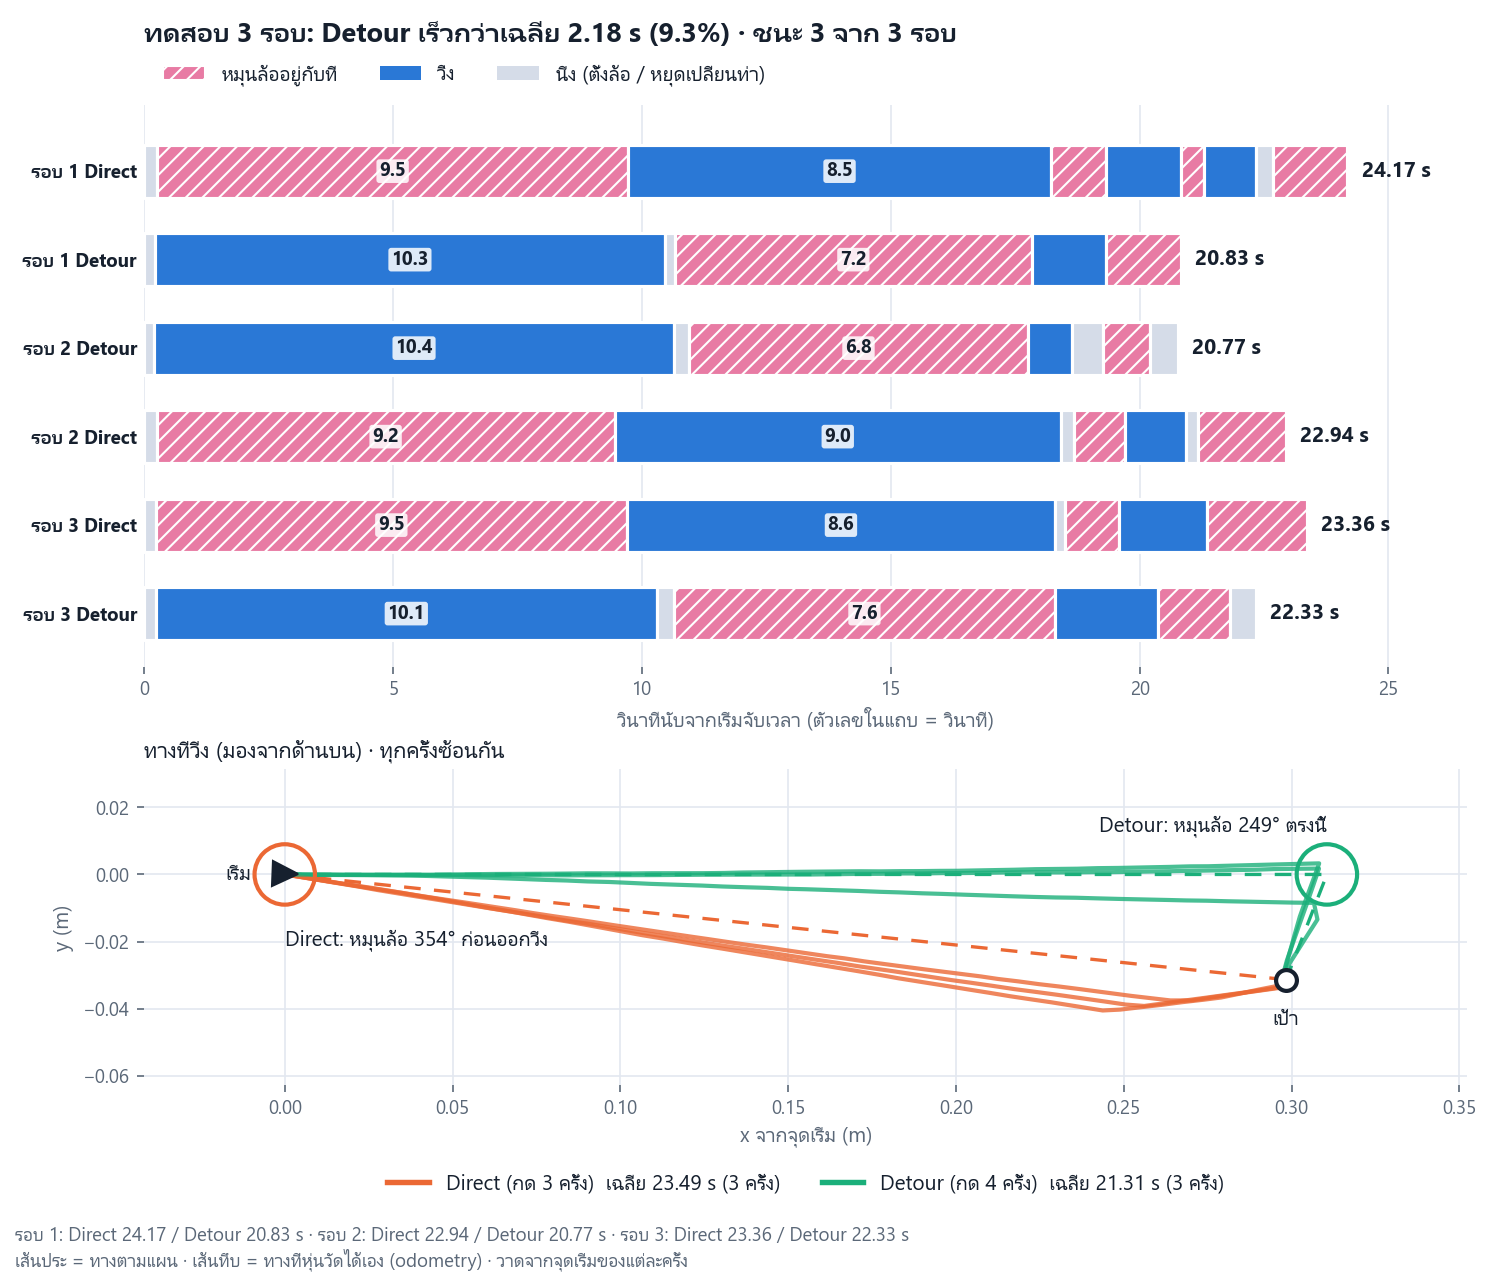
\includegraphics[width=0.93\linewidth]{robot_3rounds.png}
\end{center}
{\small
\noindent\textbf{Top:} what each run did over time (hatched pink = steering in place, blue = driving, grey =
still). The old method first steers $\approx 9.4$\,s in place, then drives; Detour Steer drives at once and
steers less later. \textbf{Bottom:} the paths the robot measured (odometry), all six from one start, seen
from above; dashed = the plan. (The robot steers counter-clockwise, so here the goal is to the right.)\par}
\vspace{1mm}
\noindent\rule{\linewidth}{1.1pt}\par


\clearpage
\section*{Current robot profile and two-metre comparison (27 October 2026)}
The numerical benchmark above uses a theoretical reference speed of 0.25 m/s;
it is not the physical robot's speed. The measured planning profile is
$v=0.03$ m/s, $\omega=35^\circ$/s, and goal radius 0.0025 m.
For the longer comparison, split a total outbound length of 2 m into seven
equal legs, each 2/7 m, bending $6^\circ$ clockwise from the preceding bearing.
Both planners visit the same waypoints; physical steering remains counter-clockwise.
The ideal model gives Direct 137.82 s / 2.00 m and Detour 110.52 s / 2.17 m,
with four detours. These are model predictions, not new real-robot measurements.
The return to start (about 1.96 m) is additional and untimed.
Three paired rounds contain six runs. No autonomous motion follows from saving settings.
\end{document}
